%!TEX root = JUrban_SOFT2014.tex

\section{Results} % (fold)
\label{sec:results}

We have selected five time slices from COMPAS shots 4275 and 6962 (i.e. 10 cases in total) for the analysis. These cases include circular, elongated and diverted plasmas with different currents. A comparison of plasma shapes for shot 4275 is shown in Fig. \ref{fig:ex4275}. Numerical values of reconstruction errors are presented in Table \ref{table:ex4275}. We can observe a very good agreement between the original equilibrium and the reconstructed shapes. In this case, FREEBIE was using linear $p'$ and $FF'$ polynomials so that the EFIT++ model agrees with the target data. VacTH uses 8 magnetic probes and 16 flux loops. As we discuss later, flux loops are essential for reliable VacTH results. Even global kinetic properties are well reconstructed in EFIT++; the largest error around 10~\% is in $l_{\mathrm i}$ (i.e. basically in the toroidal current density profile).

\begin{table*}
\centering

\begin{tabular}{lrrrrrrrrrrrrr}
\toprule
   code &  time &  $\Delta R_{\mathrm in}$ &  $\Delta R_{\mathrm out}$ &  $\Delta Z_{\mathrm min}$ &  $\Delta Z_{\mathrm max}$ &  $\delta \kappa$ &  $E_\mathrm{mp}$ &  $E_\mathrm{fl}$ &  $\delta W$ &  $\delta l_{\mathrm i}$ &  $\delta \beta_{\mathrm p}$ &  $\delta q_0$ &  $\delta q_{95}$ \\
\midrule
 EFIT++ &  0.97 &              0 &            0.002 &        0.001 &        0.001 &                  0.003 &       0.001 &      0.0009 &          0.04 &           0.09 &              0.03 &           0.03 &           0.007 \\
 EFIT++ &  0.99 &          4e-05 &            9e-05 &        0.001 &        0.001 &                  0.004 &       0.001 &      0.0006 &          0.04 &           0.09 &              0.04 &           0.02 &           0.005 \\
 EFIT++ &  1.02 &         0.0005 &           0.0002 &        0.002 &        0.002 &                  0.008 &       0.002 &       0.002 &          0.02 &            0.1 &              0.02 &           0.02 &           0.009 \\
 EFIT++ &  1.05 &          0.001 &           0.0008 &        4e-05 &       0.0003 &                  0.004 &       0.003 &       0.005 &          0.01 &           0.07 &              0.02 &           0.01 &           0.009 \\
 EFIT++ &   1.1 &          0.001 &           0.0005 &        0.005 &       0.0002 &                  0.005 &       0.004 &       0.002 &          0.04 &           0.09 &              0.03 &           0.02 &            0.05 \\
  VacTH &  0.97 &              0 &            0.001 &       0.0006 &       0.0002 &                  0.002 &       8e-07 &       7e-05 &           nan &            nan &               nan &            nan &             nan \\
  VacTH &  0.99 &          4e-05 &           0.0004 &        0.001 &       0.0008 &                  0.004 &       4e-07 &      0.0001 &           nan &            nan &               nan &            nan &             nan \\
  VacTH &  1.02 &          0.002 &           0.0008 &        0.005 &        0.002 &                   0.01 &       2e-06 &       0.002 &           nan &            nan &               nan &            nan &             nan \\
  VacTH &  1.05 &          0.006 &            0.002 &        5e-05 &        0.002 &                   0.01 &       3e-06 &        0.02 &           nan &            nan &               nan &            nan &             nan \\
  VacTH &   1.1 &          0.005 &            0.002 &        0.002 &        0.003 &                   0.02 &       2e-06 &       0.003 &           nan &            nan &               nan &            nan &             nan \\
\bottomrule
\end{tabular}

\caption{Errors for the same cases as in Fig. \ref{fig:ex4275}.}
\label{table:ex4275}
\end{table*}

\begin{figure*}
\centering   %\begin{center}
\hfill{}
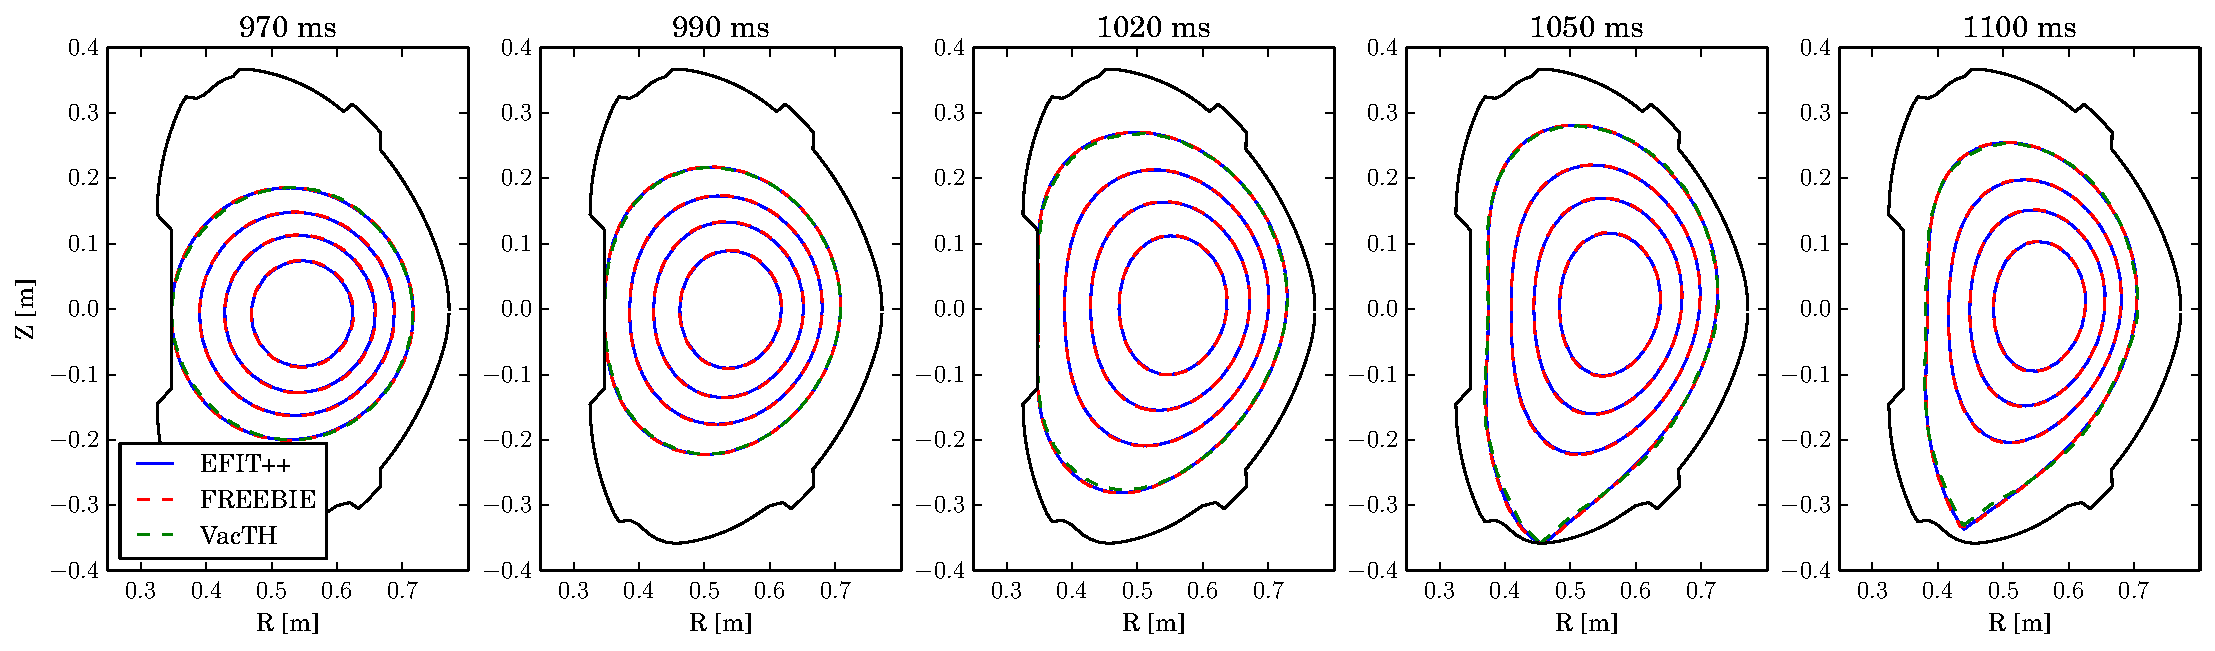
\includegraphics[width=18cm]{figures/example_4275.pdf}
\hfill{}
%\end{center}
\caption{Contours of $\bar\psi=\left(0.25,0.5,0.75,1\right)$, reconstruction from FREEBIE data, shot 4275. EFIT++ parameters: $n_\mathrm{mp} = 16$, $n_\mathrm{fl} = 4$, $n_{p'} = n_{FF'} = 1$. VacTH parameters: $n_\mathrm{mp} = 8$, $n_\mathrm{fl} = 16$, $n_{\mathrm p} = n_{\mathrm q} = 5$.}
\label{fig:ex4275}
\end{figure*}


The second shot for the comparison is 6962, which has been chosen because Thomson scattering (TS) profiles are available. On top of the same exercise as for 4275, we have calculated with FREEBIE equilibria with experimental TS pressure profiles. These equilibria of course no longer feature linear $p'$ and $FF'$ profiles.



% section results (end)
